\section{Overview}
\paragraph{}Our first sight of the system is from the highest point of view. Here we describe the architecture of the system from a \textit{layer} view.

\subsection{Three-tier-architecture}
We decided to use a \textit{three-tier-architecture} for our system.\\
A schematic representation of this responsibility distribution is at figure \ref{fig:3-tier-architecture}

\begin{figure}[H]
	\centering
	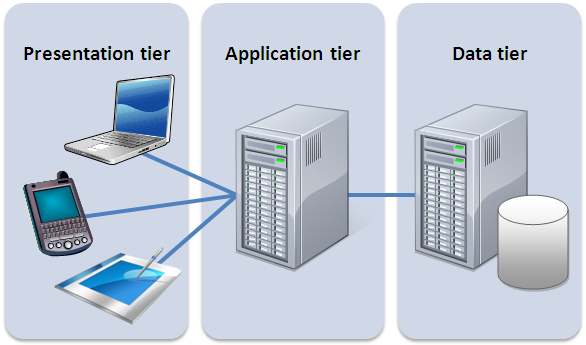
\includegraphics[scale=0.5]{../"Analysis Documents"/3-tier-architecture.png}
	\label{fig:3-tier-architecture}
	\caption{An example of three-tier-architecture}
\end{figure}
\paragraph{} So we subdivide our system in three extremely separated layers (or \textit{tiers}):
\begin{itemize}
	\item A \textit{presentation} layer for the graphic rendering of the data and events generated by the system, and from which the end user can interact with the system
	\item An \textit{application} layer entitled to manage all the business logic of the system
	\item A \textit{Data} layer responsible of the storage of informations to be used by the application and presentation layer
\end{itemize}

\subsection{An overview of our system}
\paragraph{}We can sketch our system like in figure \ref{fig:architectureOverview}
\begin{figure}
	\centering
	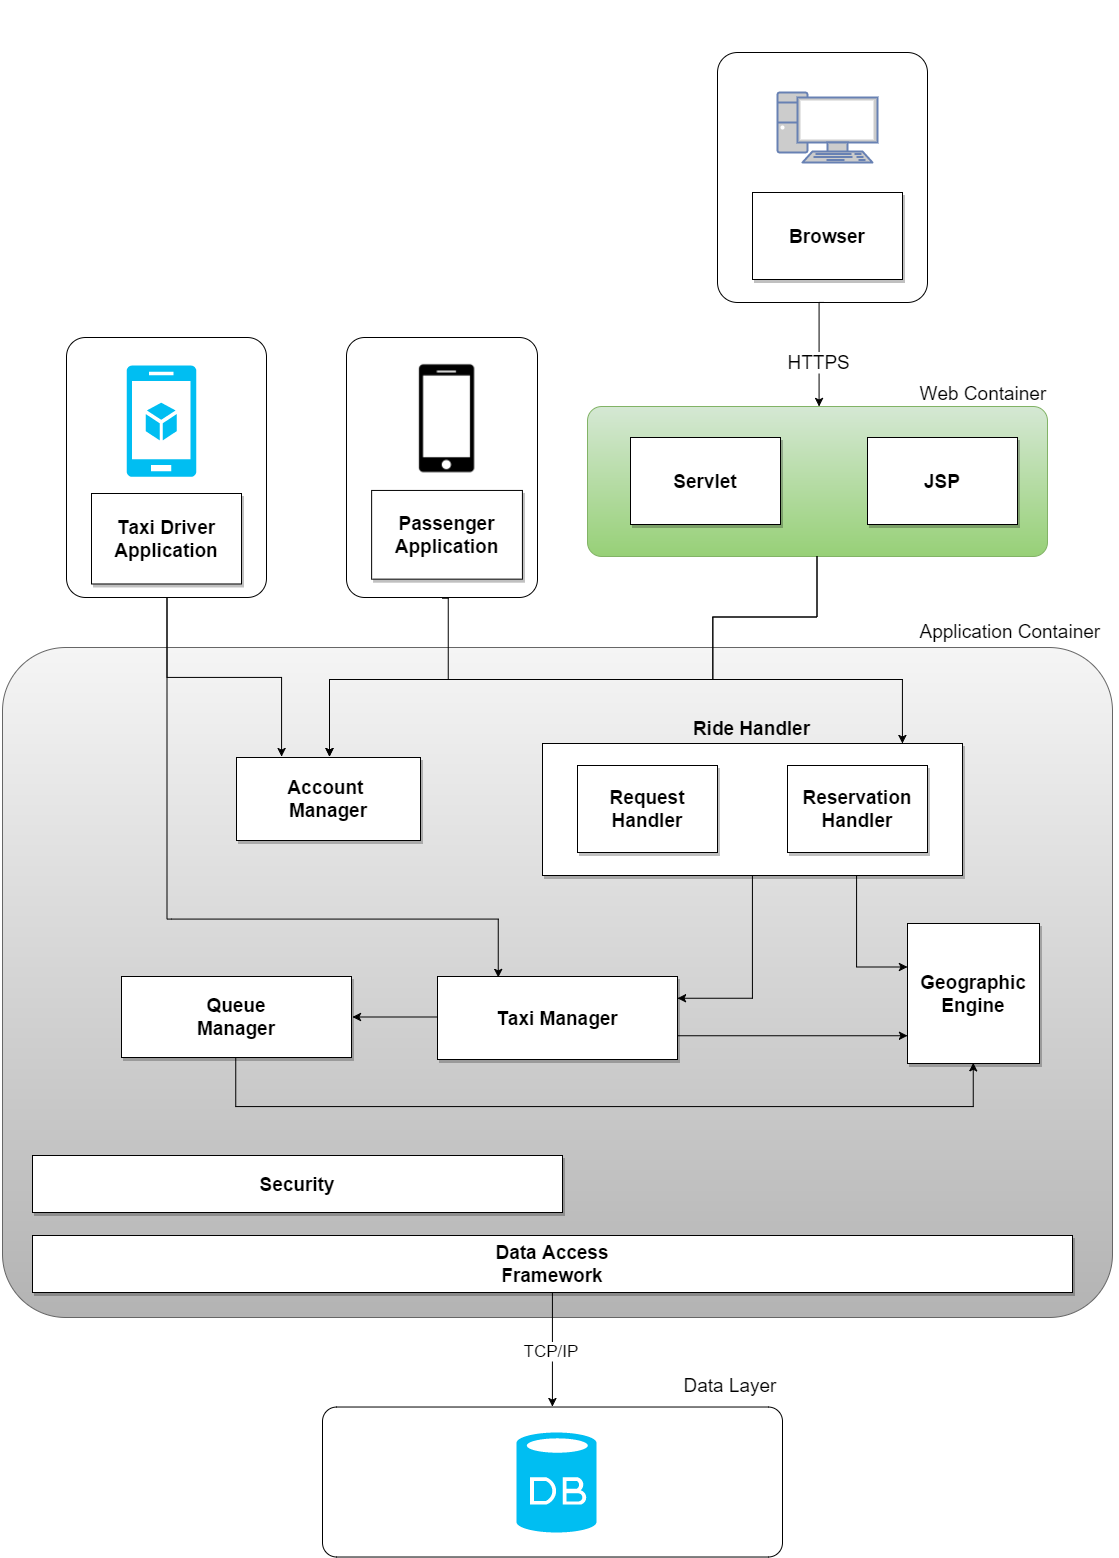
\includegraphics[scale=0.4]{../"Analysis Documents"/ArchitectureOverview.png}
	\label{fig:architectureOverview}
	\caption{Architecture Overview}
\end{figure}